基数排序(Radix
sort)是一种非比较型整数排序算法,其原理是{将整数按位数切割成不同的数字,然后按每个位数分别比较}。由于整数也可以表达字符串(比如名字或日期)和特定格式的浮点数,所以基数排序也不是只能使用于整数。

将所有待比较数值(正整数)统一为同样的数位长度,数位较短的数前面补零。然后,从最低位开始,依次进行一次排序。这样从最低位排序一直到最高位排序完成以后,数列就变成一个有序序列。

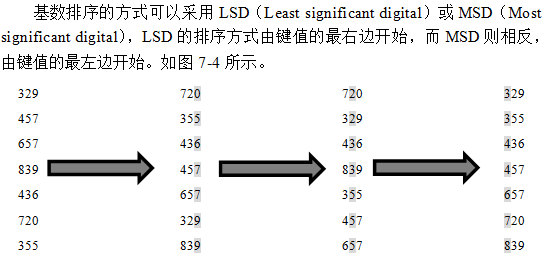
\includegraphics[width=3.70833in,height=1.77083in]{png-jpeg-pics/A5BBC1816F49FFEDC5AFA6AC3CA4666D.png}

{关于这个算法,很重要的一点就是按位排序更稳定。否则排序会出错。}

{\textbf{算法分析:}}{给定n个d位数,每一个数位可以取k种可能的值,如果所用的稳定排序需要O(n+k)的时间。则平均和最坏时间复杂度都为O(d(n+k))。空间复杂度为O(k)。}{}
